\chapter{Background}





\section{Theory }
In this section we highlight fundamental concepts and information needed for the thesis.
\subsection{Android : System and Performance Constraints}
%https://source.android.com/source/index.html
%https://source.android.com/compatibility/index.html
%https://android.googlesource.com/platform/frameworks/base/+/master/core/res/res/xml/power_profile.xml
%https://source.android.com/devices/tech/power/index.html#power-values
%https://source.android.com/devices/tech/power/index.html
%http://www.tutorialspoint.com/android/android_architecture.htm
%https://developer.android.com/tools/performance/index.html - important
Android\texttrademark{} is an open source system software stack, built on top of the Linux kernel, that provides services and supports variety of (mobile) devices. Figure \ref{fig:androidstack} shows the Android software stack  and figure  \ref{fig:androidarch} shows the architecture of the Android operating system that are referred by applications developers, hardware developers, Original Equipment Manufactures (OEM) and carriers. This leads to variety of customizations and uncontrolled customization would result in incompatible implementations. Hence, Android tightly integrate OEMs with the \textit{Android Compatibility program}, developers with \emph{Android SDK}, users with \emph{Google Play}. For this thesis only devices with the compatible Android ecosystem is considered.

\begin{figure}[h]	
	\centering
	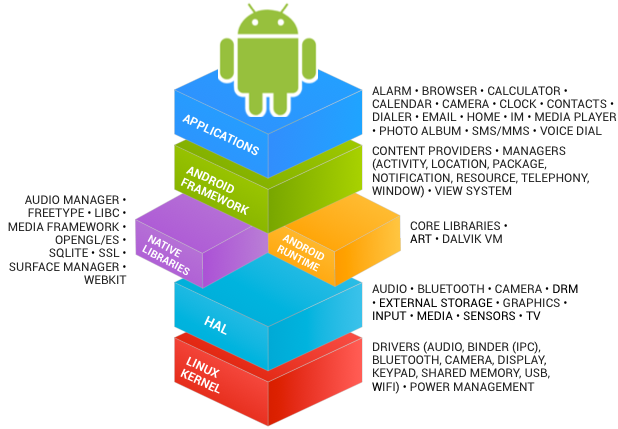
\includegraphics[width=0.9\textwidth]{Figures/c1framework.png}
	\caption{Android Stack \small(https://source.android.com)}
	 \label{fig:androidstack}
\end{figure} 

\begin{figure}[h]
	\begin{center}	
	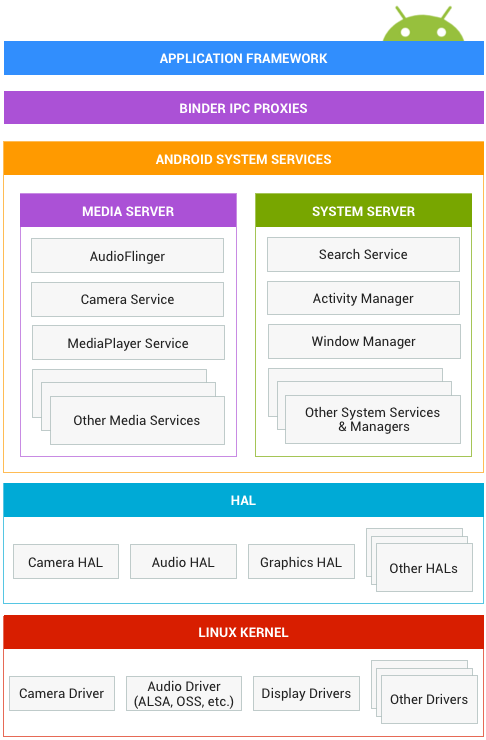
\includegraphics[width=0.7\textwidth]{Figures/c1architecture.png}
   \end{center}
	\caption{Android System Architecture \small(https://source.android.com)}
	\label{fig:androidarch}
\end{figure} 

\subsubsection*{Rendering}
This 


\subsection{Energy Profiling}
external, utilization-based, system call level
\subsection{Energy Models}
mathematical
\subsection{Energy Drain Prediction}
\subsection{Crowd Sourcing}
\subsection{Big Data Analysis}
\subsection{Data communications}
\subsection{Cloud Architectures}
Amazon , Google Compute, Heroku
\section{Related Works and Interesting Results}
There has been many efforts made to enable energy efficiency in smart-phones and in IoT in general. They are a range of solutions tried out in \emph{Hardware Architecture} level \cite{EE:MCCarch,EE:JVM}, \emph{Data communication} level \cite{EE:eTime,EE:Multinets},  \emph{Network infrastructure} level \cite{EE:Hier} and in \emph{Protocols} optimization \cite{EE:Protocol}. As Intel summed up in \cite{EE:GreenSW}, \emph{Software Energy Efficiency} is towards achieving \emph{Computational Efficiency}, \emph{Data Efficiency}, \emph{Context Awareness} and \emph{Idle Efficiency} in broader sense. Few common problems with most of the existing solutions are including: 1) system as a whole was not considered;
2) trade-off between components was not properly considered;
3) interdependences of the components was not properly studied;
4) the existing solutions are suboptimal. For measuring energy consumption, solid background has been provided  in \cite{EE:Measure}. Internet of Things-Architecture, a consortium is rigorously developing architectural reference models. The models could potentially serve the best initial  guidance towards concrete architecture for the problem of interest and eventually towards the actual system architecture \cite{IoTA:ARM}. In \cite{Orches:Arch}, devices orchestration is explained in business process point of view.
%%%%%%%%%%%%% Extra %%%%
%\begin{wrapfigure}{l}{0.3\textwidth}
% \begin{center}
%  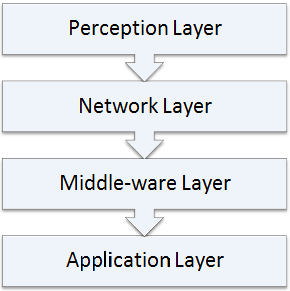
\includegraphics[scale=0.30]{Figures/IoTArch.png}
% \end{center}
% \caption{IoT Architecture}
%\end{wrapfigure}

%\begin{figure}[H]
% \begin{center}
%  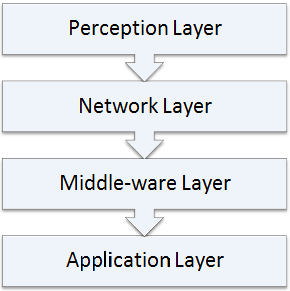
\includegraphics[scale=0.30]{Figures/IoTArch.png}
% \end{center}
% \caption{IoT Architecture}
%\end{figure}

% \cite{EE:Protocol,EE:Hier,EE:RedunData,EE:Diagnosis,
% EE:Measure,EE:MeasureWiFi,EE:Perform,EE:GreenSW,EE:Eaware}